\chapter*{Wprowadzenie}
\addcontentsline{toc}{chapter}{Wprowadzenie}
% jaka będzie wartość dodana tego co zrobimy
% cała ścieżka Informatyka -> nasza praca
% celem naszym było usystematyzować pracę nad systemami dla sumerologów

% nasza ścieżka: Informatyka -> Inżynieria oprogramowania -> różne podejścia -> domain-specific podejście -> domain specific language
 

% 1. krótki opis problemu - są sumerolodzy, mają tabliczki, chcą sprawnie wyszukiwać
\section*{Opis problemu}
Ok. 3500 lat przed naszą erą starożytni Sumerowie, jako prawdopodobnie pierwsi na świecie, zaczęli używać pisma. 
Ze względu na ksztat liter odciśniętych za pomocą trzciny w miękkiej glinie zostało ono później nazwane pismem klinowym. 
Sumerowie używali go głównie w celach administracyjnych. Zapisywali między innymi rachunki za dostawy zwierząt oraz rozliczenia z 
wykonanej na polu lub w warsztacie pracy i należnej zapłaty. Jednymi z ciekawszych tekstów są tzw. listy królów, na 
których znajdują się daty panowania kolejnych władców i ich osiągnięcia w poszczególnych latach. 
Ważniejsze tabliczki wypalano, jednak większość po pewnym czasie niszczono, aby zużytą glinę można było ponownie wykorzystać. 
Do dzisiaj przetrwały głównie te tabliczki, które zostały wypalone podczas przypadkowego pożaru archiwum. 
Wiele z nich jest zniszczonych, jednak wciąż stanowią ogromną wartość historyczną. 
 
Na podstawie zachowanych tabliczek można się wiele dowiedzieć o historii Sumeru, a także o życiu zwykłych ludzi w tym okresie, 
o ich zarobkach, zasiłkach i dniach wolnych. Odczytywaniem tych informacji zajmują się sumerolodzy z całego świata. 
Aby łatwiej dzielić się zdobytą wiedzą, zaczęli tworzyć cyfrowe bazy tabliczek, dostępne w internecie. 
Największa z nich to Cuneiform Digital Library Initiative (CDLI), zawierająca prawie 225 tys tekstów.

Jednak wyszukiwanie interesujących tabliczek może być w tym momencie uciążliwe. 

Sumerolodzy mogliby skorzystać ze specyficznych dla baz danych języków zapytań (np. SQL), ale po pierwsze większość z 
nich nie zna tych języków, a po drugie budowanie w ten sposób złożonych zapytań dotyczących danych tekstowych jest czasochłonne. 
Takie języki były tworzone z myślą o bardziej generycznych zastosowaniach i nie odpowiadają potrzebom sumerologów.
Z tych powodów większość istniejących obecnie serwisów internetowych udostępnia formularze ułatwiające wprowadzanie kryteriów
 wyszukiwania. Jednak mają one ograniczone możliwości i nie pozwalają na konstruowanie bardziej skomplikowanych zapytań.
Dlatego istnieje potrzeba stworzenia narzędzia wspomagającego wyszukiwanie, które będzie łączyło w sobie jak największ siłę 
wyrazu oraz łatwość użycia dla osób znających jedynie dziedzinę problemu.

% 2. różne podejścia do tworzenia oprogramowania
Przy tego typu problemach z pomocą przychodzi informatyka. 

\section*{Propozycja rozwiązania}
Do tej pory powstało wiele różnych systemów informatycznych, a doświadczenie stopniowo zdobywane przy ich budowie prowadzi do 
ciągłego rozwijania nauki zwanej inżynierią oprogramowania, zajmującej się praktyczną stroną wytwarzania systemów. Obecnie jest 
znanych bardzo wiele podejść do tworzenia oprogramowania, a każdemu odpowiada gałąź problemów, w których sprawdza się najlepiej. 
% Część z nich rozważałyśmy zastanawiająć się nad problemem sumerologów.

Najbardziej popularne jest programowanie zorientowane obiektowo (ang. \emph{Object-Oriented Programming}, OOP), które polega na modelowaniu 
świata rzeczywistego w postaci \textit{obiektów}. Obiekty posiadają dane oraz metody, które mogą te dane zmieniać. Program jest zbiorem 
obiektów komunikujących się między sobą. 

Innym podejściem jest architektura zorientowana na usługi (ang. \emph{Service-Oriented Architecture}, SOA), w której definiuje się 
niezależne od siebie usługi (services) i udostępnia tylko ich interfejsy, ukrywając implementację.

Rozważając problem sumerologów zdecydowałyśmy się na programowanie zorientowane na język (ang. \emph{Language-Oriented Programming}). 
Polega ono na stworzeniu języka odpowiadającego dziedzinie problemu, czyli tzw. języka dziedzinowego (ang. \emph{Domain-Specific Language},
 DSL). Dopiero w tym nowym języku rozwiązuje się konkretny problem (np. znalezienie tekstów sumeryjskich z epoki Ur III dotyczących owiec). 
Opisywanie problemów dziedziny jest wtedy znacznie prostsze i bardziej naturalne, a dzięki temu wygodne dla ludzi związanych tylko z 
konkretną dziedziną. 

Wyróżnia się dwa rodzaje języków dziedzinowych - ``wewnętrzne`` (ang. \emph{internal}), które zachowują składnię istniejących już języków 
i ograniczają tylko ich możliwości, oraz ``zewnętrzne`` (ang. \emph{exernal}), które są zupełnie nowymi językami, tłumaczonymi do 
istniejących wcześniej \cite{fowler}. W naszym przypadku narzucającym się podejściem było stworzenie nowego, zewnętrznego DSL, zaprojektowanego 
specjalnie do wyszukiwania tabliczek sumeryjskich, który miałby składnię przejrzystą dla sumerologa. 

% 3. wybrałyśmy takie podejście bo...
% Zazwyczaj do konkretnego problemu jedno z podejść pasuje zdecydowanie bardziej niż inne. W niniejszej pracy zdecydowałyśmy się zastosować programowanie zorientowane na język w celu usystematyzowania pracy nad systemami dla sumerologów. 
Do każdej bazy zawierającej tabliczki można skonstruować moduł pozwalający na wyszukiwanie z użyciem takiego DSL.
Zatem jest to rozwiązanie, które może zostać wykorzystane przez wiele różnych serwisów, zarówno nowo powstających, jak i tych już 
istniejących. Dzięki temu wyszukiwarki, internetowe oraz stacjonarne, mogłyby mieć taki sam lub bardzo podobny interferjs, co znacznie 
ułatwiłoby pracę sumerologom. DSL pozwoliłby usystematyzować prace nad wszelkimi wyszukiwarkami tabliczek sumeryjskich, a przez to również 
pracę sumerologów. Jest to niewątpliwa zaleta takiego rozwiązania. Wyraźnie widać jego przewagę nad podejściem polegającym na niezależnym 
rozwijaniu interfejsów poszczególnych wyszukiwarek, czego efektem są coraz bardziej skomplikowane formularze do wpisywania zapytań.


\section*{Tablets Query Language}

% 4. troszkę o TQL-u
Wychodząc naprzeciw potrzebom sumerologów prezentujemy stworzony przez nas język dziedzinowy do wyszukiwania tabliczek sumeryjskich --- 
\textit{Tablets Query Language} (TQL). Został on zaprojektowany przede wszystkim jako intuicyjny i zrozumiały dla osób z dziedziny problemu.
 Ma także minimalnie ograniczać siłę wyrazu tzn. pozwalać na konstruowanie jak najbardziej skomplikowanych zapytań. Chcemy również, żeby 
był niezależny od sposobu reprezentacji tabliczek. W niniejszej pracy udowodnimy, że TQL spełnia wszystkie te wymagania. 

% TODO: przerobić - wziąć wzroce z When and how i przeformułować
% design pattern - language invention
% implementation pattern - preprocesor => source to source
Zgodnie z paradygmatem języka dziedzinowego, TQL jest tłumaczony do innych, istniejących wcześniej języków zapytań bardziej 
ogólnego zastosowania, np. SQL, XQuery \cite{xquery}, odpowiednio do sposobu reprezentacji danych.


Sposobem reprezentacji danych nazywamy rodzaj bazy danych (np. relacyjna, obiektowa, XML), konkretną implementację serwera 
(np. PostgreSQL \cite{postgres}, Zorba \cite{zorba}) oraz schemat danych. Dla każdego takiego sposobu zapytanie w docelowym jzyku może się różnić, a zatem 
różnić się będzie również program tłumaczący TQL na ten język.
Oznacza to, że dla każdego sposobu reprezentacji danych należy stworzyć oddzielny program tłumaczący. 
%którego zadaniem będzie przetłumaczenie zapytania na odpowiedni do tej reprezentacji język. 
W ramach niniejszej pracy oprócz języka TQL zaprezentujemy dwie prototypowe implementacje komponentu do wyszukiwarki, zawierającego 
m.in. program tłumaczący.
Ten komponent, nazywany dalej w translatorem, tłumaczy zapytanie TQL na zapytanie w języku specyficznym dla danej bazy, przekazuje 
przetłumaczone zapytanie do bazy, odbiera wynik i przedstawia go w odpowiedniej postaci. Pokażemy implementacje translatora dla bazy 
PostgreSQL (z językiem wyszukiwania SQL) oraz dla bazy XML (z językiem wyszukiwania XQuery).
% Celem projektu przedstawionego w niniejszej pracy jest zaprojektowanie i implementacja takiego języka, który nazwałyśmy Tablets Query Language (TQL). Ma być intuicyjny i zrozumiały dla sumerologów, umożliwiając jednocześnie tworzenie skomplikowanych zapytań.
% Będzie on udostępniał wyszukiwanie po różnych parametrach tabliczki. 


% Dla każdego z nich, w zależności od reprezentacji danych, należy skonstruować translator, 
% którego zadaniem będzie przetłumaczenie zapytania. 
%W ramach niniejszej pracy przedstawione zostaną dwa przykładowe translatory.



TQL może być także podstawą do tworzenia podobnych języków wyszukiwań dostosowanych do potrzeb innych grup ludzi, np. językoznawców.
Większość programów ułatwiających tworzenie zapytań jest skomplikowana, daje ograniczone możliwości lub jest przystosowana głównie do 
przetwarzania danych liczbowych. Tablets Query Language rozwiązuje te problemy: jest prosty i intuicyjny, przystosowany głównie do tekstów,
 minimalnie zmniejsza siłę wyrazu oraz łatwo go rozbudowywać. 




%  \begin{figure}
%   \centering
% \includegraphics[width=340px]{./diagramy/poco.pdf}
%   \caption{Zarysowanie problemu}
%  \end{figure}
\begin{figure}[h]
 \centering
 \includegraphics[width=400px]{../diagramy/poco.pdf}
 % poco.pdf: 596x842 pixel, 72dpi, 21.03x29.70 cm, bb=0 0 596 842
 \caption{Przedstawienie problemu}
 \label{fig:poco}
\end{figure}

